\documentclass{beamer}\usepackage[]{graphicx}\usepackage[]{color}
%% maxwidth is the original width if it is less than linewidth
%% otherwise use linewidth (to make sure the graphics do not exceed the margin)
\makeatletter
\def\maxwidth{ %
  \ifdim\Gin@nat@width>\linewidth
    \linewidth
  \else
    \Gin@nat@width
  \fi
}
\makeatother

\definecolor{fgcolor}{rgb}{0.345, 0.345, 0.345}
\newcommand{\hlnum}[1]{\textcolor[rgb]{0.686,0.059,0.569}{#1}}%
\newcommand{\hlstr}[1]{\textcolor[rgb]{0.192,0.494,0.8}{#1}}%
\newcommand{\hlcom}[1]{\textcolor[rgb]{0.678,0.584,0.686}{\textit{#1}}}%
\newcommand{\hlopt}[1]{\textcolor[rgb]{0,0,0}{#1}}%
\newcommand{\hlstd}[1]{\textcolor[rgb]{0.345,0.345,0.345}{#1}}%
\newcommand{\hlkwa}[1]{\textcolor[rgb]{0.161,0.373,0.58}{\textbf{#1}}}%
\newcommand{\hlkwb}[1]{\textcolor[rgb]{0.69,0.353,0.396}{#1}}%
\newcommand{\hlkwc}[1]{\textcolor[rgb]{0.333,0.667,0.333}{#1}}%
\newcommand{\hlkwd}[1]{\textcolor[rgb]{0.737,0.353,0.396}{\textbf{#1}}}%
\let\hlipl\hlkwb

\usepackage{framed}
\makeatletter
\newenvironment{kframe}{%
 \def\at@end@of@kframe{}%
 \ifinner\ifhmode%
  \def\at@end@of@kframe{\end{minipage}}%
  \begin{minipage}{\columnwidth}%
 \fi\fi%
 \def\FrameCommand##1{\hskip\@totalleftmargin \hskip-\fboxsep
 \colorbox{shadecolor}{##1}\hskip-\fboxsep
     % There is no \\@totalrightmargin, so:
     \hskip-\linewidth \hskip-\@totalleftmargin \hskip\columnwidth}%
 \MakeFramed {\advance\hsize-\width
   \@totalleftmargin\z@ \linewidth\hsize
   \@setminipage}}%
 {\par\unskip\endMakeFramed%
 \at@end@of@kframe}
\makeatother

\definecolor{shadecolor}{rgb}{.97, .97, .97}
\definecolor{messagecolor}{rgb}{0, 0, 0}
\definecolor{warningcolor}{rgb}{1, 0, 1}
\definecolor{errorcolor}{rgb}{1, 0, 0}
\newenvironment{knitrout}{}{} % an empty environment to be redefined in TeX

\usepackage{alltt}

\usepackage{alltt}%
\usetheme{Boadilla}
\usecolortheme{seahorse}

\usepackage[utf8]{inputenc}
\usepackage{default}

\usepackage{xcolor}%for color mixing

\usepackage{amsmath}%
\usepackage{amsfonts}%
\usepackage{amssymb}%
\usepackage{graphicx}

\usepackage{tikz}
\usepackage{multirow}
\usepackage{booktabs}

\setbeamertemplate{itemize/enumerate body begin}{\small}

\usepackage{hyperref}

%%%%%%%%%%%%%%%%%%%%%%%%%%%%%%%%%%%%%%%%%%%%%%%%%%%%%%%%%%%%%%%%%%%%%%%%%%%%%%%%%%

\title{Programming with functions in R}
\subtitle{Useful things, funny things and stat theory}
\author{Timoth\'ee Bonnet}
\date{\today}
\IfFileExists{upquote.sty}{\usepackage{upquote}}{}
\begin{document}

%\lstset{language=R}%code

\AtBeginSection[]
{
  \begin{frame}<beamer>
    \frametitle{}
    \tableofcontents[currentsection,sectionstyle=show/show,subsectionstyle=show/shaded/hide]% down vote\tableofcontents[currentsection,currentsubsection,hideothersubsections,sectionstyle=show/hide,subsectionstyle=show/shaded/hide] 
  \end{frame}
}

\begin{frame}{}%pre-start slide0
\centering
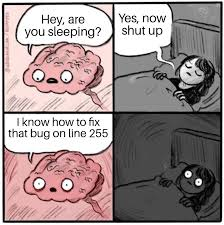
\includegraphics[width=0.35\textwidth]{figures/images.jpeg}
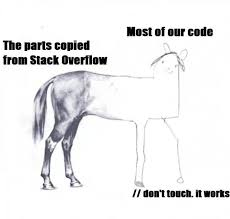
\includegraphics[width=0.35\textwidth]{figures/images2.jpeg}

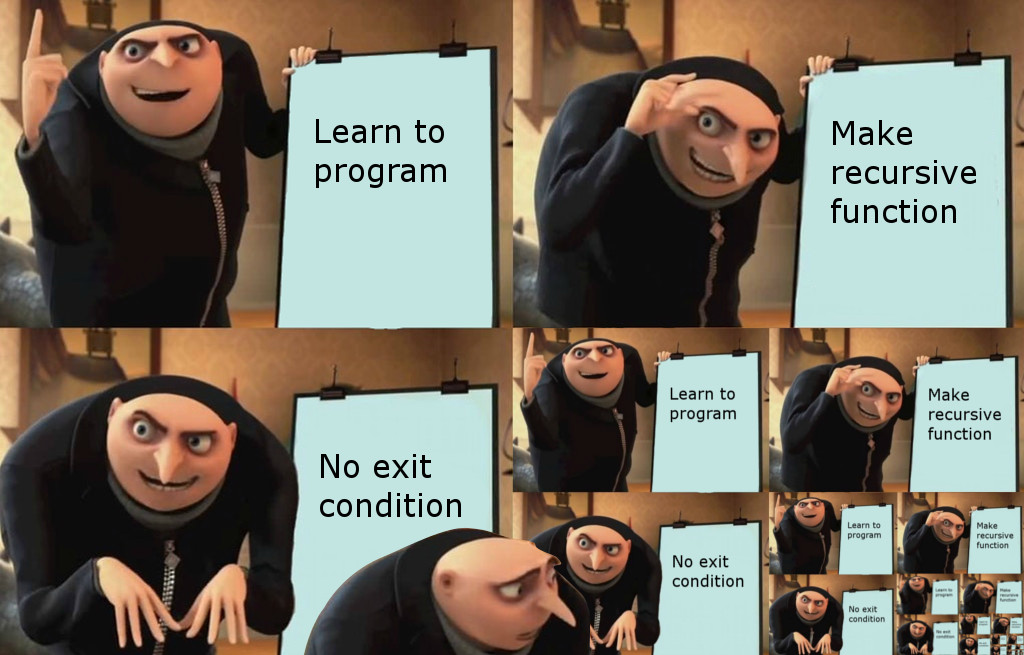
\includegraphics[width=0.45\textwidth]{figures/recursive}\\ That last one will make sense in 2h
\end{frame}
%%%%%%%%%%%%

\begin{frame}
  \maketitle
\end{frame}

\section{Functions and where to find them}

\begin{frame}{Why make your own functions?}
  
\begin{block}{Pros}
  \begin{itemize}
    \item Less code writing
    \item Fewer mistakes
    \item Cleaner code
    \item More transferable code
  \end{itemize}
  Hence reproducibility and mental health
\end{block}  

\pause

\begin{alertblock}{Cons}
  \begin{itemize}
    \item More thinking
    \item Not always worth time investment
  \end{itemize}
\end{alertblock}

\end{frame}
%%%%%%%%%%%


\begin{frame}[fragile]{Anatomy of a function}

What is inside a function?
\begin{knitrout}
\definecolor{shadecolor}{rgb}{0.969, 0.969, 0.969}\color{fgcolor}\begin{kframe}
\begin{alltt}
  \hlstd{mean}
  \hlstd{apply}
\end{alltt}
\end{kframe}
\end{knitrout}

\pause
Hmm, clearer information?
\begin{knitrout}
\definecolor{shadecolor}{rgb}{0.969, 0.969, 0.969}\color{fgcolor}\begin{kframe}
\begin{alltt}
  \hlopt{?}\hlstd{apply}
  \hlopt{?}\hlkwd{apply}\hlstd{()}
\end{alltt}
\end{kframe}
\end{knitrout}
\pause

\begin{block}{Lots of code in one word}
\end{block}
\end{frame}
%%%%%%%%%%%%

\begin{frame}[fragile]{How to make a function}

\begin{knitrout}
\definecolor{shadecolor}{rgb}{0.969, 0.969, 0.969}\color{fgcolor}\begin{kframe}
\begin{alltt}
\hlstd{myfunction} \hlkwb{<-} \hlkwa{function}\hlstd{()\{}
  \hlnum{3}\hlopt{+}\hlnum{5}
\hlstd{\}}

\hlkwd{myfunction}\hlstd{()}
\end{alltt}
\begin{verbatim}
## [1] 8
\end{verbatim}
\end{kframe}
\end{knitrout}

\texttt{myfunction} is now an object in the environment
\end{frame}
%%%%%%%%%%%%

\begin{frame}[fragile]{Input/output}

\begin{block}{}
  \begin{itemize}
  \item Zero to many input objects (Arguments)
  \item Return one object (Value)
  \end{itemize}
\end{block}

\begin{knitrout}
\definecolor{shadecolor}{rgb}{0.969, 0.969, 0.969}\color{fgcolor}\begin{kframe}
\begin{alltt}
  \hlkwd{mean}\hlstd{(}\hlkwc{x} \hlstd{=} \hlkwd{c}\hlstd{(}\hlnum{3}\hlstd{,}\hlnum{7}\hlstd{,}\hlnum{1}\hlstd{),} \hlkwc{na.rm} \hlstd{=} \hlnum{TRUE}\hlstd{)}
\end{alltt}
\end{kframe}
\end{knitrout}

\pause
\begin{knitrout}
\definecolor{shadecolor}{rgb}{0.969, 0.969, 0.969}\color{fgcolor}\begin{kframe}
\begin{alltt}
\hlstd{myfunction} \hlkwb{<-} \hlkwa{function}\hlstd{(}\hlkwc{x}\hlstd{,} \hlkwc{y}\hlstd{)\{}
  \hlstd{x}\hlopt{+}\hlstd{y}
\hlstd{\}}

\hlkwd{myfunction}\hlstd{(}\hlnum{2}\hlstd{,} \hlnum{4}\hlstd{);} \hlkwd{myfunction}\hlstd{(}\hlnum{3}\hlstd{,} \hlnum{5}\hlstd{)}
\end{alltt}
\begin{verbatim}
## [1] 6
## [1] 8
\end{verbatim}
\end{kframe}
\end{knitrout}

\texttt{myfunction} now takes two arguments

\end{frame}
%%%%%%%%%%%%%%


\begin{frame}[fragile]{Input/output}

\begin{block}{}
  \begin{itemize}
  \item Zero to many input objects (Arguments)
  \item Return one object (Value)
  \end{itemize}
\end{block}

\begin{knitrout}
\definecolor{shadecolor}{rgb}{0.969, 0.969, 0.969}\color{fgcolor}\begin{kframe}
\begin{alltt}
\hlstd{myfunction} \hlkwb{<-} \hlkwa{function}\hlstd{(}\hlkwc{x}\hlstd{,} \hlkwc{y}\hlstd{)\{}
  \hlstd{x}\hlopt{-}\hlstd{y}
  \hlstd{x}\hlopt{+}\hlstd{y}
\hlstd{\}}

\hlkwd{myfunction}\hlstd{(}\hlnum{2}\hlstd{,} \hlnum{4}\hlstd{);} \hlkwd{myfunction}\hlstd{(}\hlnum{3}\hlstd{,} \hlnum{5}\hlstd{)}
\end{alltt}
\begin{verbatim}
## [1] 6
## [1] 8
\end{verbatim}
\end{kframe}
\end{knitrout}

\textbf{Functions returns only the result from the last line by default}
\end{frame}
%%%%%%%%%%%%%



\begin{frame}[fragile]{Input/output}

\begin{block}{}
  \begin{itemize}
  \item Zero to many input objects (Arguments)
  \item Return one object (Value)
  \end{itemize}
\end{block}

\begin{knitrout}
\definecolor{shadecolor}{rgb}{0.969, 0.969, 0.969}\color{fgcolor}\begin{kframe}
\begin{alltt}
\hlstd{myfunction} \hlkwb{<-} \hlkwa{function}\hlstd{(}\hlkwc{x}\hlstd{,} \hlkwc{y}\hlstd{)\{}
  \hlstd{subvalue} \hlkwb{<-} \hlstd{x}\hlopt{-}\hlstd{y}
  \hlstd{advalue} \hlkwb{<-} \hlstd{x}\hlopt{+}\hlstd{y}
  \hlkwd{return}\hlstd{(subvalue)}
  \hlstd{x}\hlopt{*}\hlstd{y}
\hlstd{\}}

\hlkwd{myfunction}\hlstd{(}\hlnum{2}\hlstd{,} \hlnum{4}\hlstd{);} \hlkwd{myfunction}\hlstd{(}\hlnum{3}\hlstd{,} \hlnum{5}\hlstd{)}
\end{alltt}
\begin{verbatim}
## [1] -2
## [1] -2
\end{verbatim}
\end{kframe}
\end{knitrout}

\textbf{Functions returns only \texttt{return()} is one is provided}
\end{frame}
%%%%%%%%%%%%%

\begin{frame}{Exercise 1 and 2}

\begin{enumerate}
  \item Write a function that return the product of three arbitrary numbers together (x*y*z) provided by the user
  \item Write a function that return the product of three arbitrary numbers together (x*y*z) as well as their sum (x+y+z)
\end{enumerate}

\end{frame}
%%%%%%%%%%%

\begin{frame}{Scope}
"What happens in Functions Stays in Functions" (unless\dots)

\begin{knitrout}
\definecolor{shadecolor}{rgb}{0.969, 0.969, 0.969}\color{fgcolor}\begin{kframe}
\begin{alltt}
\hlstd{x} \hlkwb{<-} \hlnum{10}

\hlstd{myfunction} \hlkwb{<-} \hlkwa{function}\hlstd{(}\hlkwc{x}\hlstd{)\{}
  \hlstd{x} \hlkwb{<-} \hlnum{5}
\hlstd{\}}

\hlkwd{myfunction}\hlstd{(}\hlkwc{x}\hlstd{=x)}

\hlstd{x}
\end{alltt}
\end{kframe}
\end{knitrout}
What is the value of x ?

\end{frame}
%%%%%%%%%%%%


\begin{frame}[fragile]{Scope}
"What happens in Functions Stays in Functions" (unless\dots)

Save the output to an object
\begin{knitrout}
\definecolor{shadecolor}{rgb}{0.969, 0.969, 0.969}\color{fgcolor}\begin{kframe}
\begin{alltt}
\hlstd{x} \hlkwb{<-} \hlnum{10}
\hlstd{x} \hlkwb{<-} \hlkwd{myfunction}\hlstd{(}\hlkwc{x}\hlstd{=x)}
\hlstd{x}
\end{alltt}
\begin{verbatim}
## [1] 5
\end{verbatim}
\end{kframe}
\end{knitrout}

\pause

Or special functions to break environment boundaries (Scoping assignment, see later)

\end{frame}

%%%%%%%%%%%%%%%%%%%%%%%%%%%%%%%%%%%%%%%%%%%%%
\begin{frame}[fragile]{Sourcing as "primitive package"}

Do Exercise 3

\pause
\textbf{Complex code can easily be turned into a function}

\pause
\vfill
Save the function you just made to a new file "myfunctions.R".\\
You can now call ("source") this file and all the functions it contains: 
\begin{knitrout}
\definecolor{shadecolor}{rgb}{0.969, 0.969, 0.969}\color{fgcolor}\begin{kframe}
\begin{alltt}
\hlkwd{source}\hlstd{(}\hlstr{"myfunctions.R"}\hlstd{)}
\end{alltt}
\end{kframe}
\end{knitrout}


\end{frame}
%%%%%%%%%%%%

\begin{frame}{Fun time: Big exercise and stat theory!}

\textbf{Exercise 4!}

\end{frame}

\section{Funny things}

\begin{frame}[fragile]{Lists of functions!}

\begin{knitrout}
\definecolor{shadecolor}{rgb}{0.969, 0.969, 0.969}\color{fgcolor}\begin{kframe}
\begin{alltt}
\hlstd{funs} \hlkwb{<-} \hlkwd{list}\hlstd{(}
  \hlkwc{half} \hlstd{=} \hlkwa{function}\hlstd{(}\hlkwc{x}\hlstd{) x} \hlopt{/} \hlnum{2}\hlstd{,}
  \hlkwc{double} \hlstd{=} \hlkwa{function}\hlstd{(}\hlkwc{x}\hlstd{) x} \hlopt{*} \hlnum{2}
\hlstd{)}
\hlstd{funs}\hlopt{$}\hlkwd{double}\hlstd{(}\hlnum{10}\hlstd{)}
\end{alltt}
\begin{verbatim}
## [1] 20
\end{verbatim}
\end{kframe}
\end{knitrout}
\end{frame}
%%%%%%%%%%%


\begin{frame}{The dot-dot-dot}
\textbf{See exercise 5}

\end{frame}
%%%%%%%%%%%%

\begin{frame}[fragile]{Scoping assignment}
Using \texttt{<<-} or \texttt{assign(x, value, inherits=TRUE)}

\textbf{See exercise 6}

Can be difficult, but can be useful (e.g. functions that create functions)
\end{frame}
%%%%%%%%%%%

\begin{frame}[fragile]{Recursive function}

A function can call another function, including itself\\
\textbf{See Exercises 7 and 8}

\end{frame}
%%%%%%%%%%%


\begin{frame}{To go further}
Everything you (didn't) want to know about functions in R: \url{https://adv-r.hadley.nz/functions.html\#introduction-5}


\end{frame}
%%%%%%%%%%%

\end{document}
